\documentclass[10pt]{article}
\usepackage[a4paper,margin=18mm]{geometry}
\usepackage[T1]{fontenc}\usepackage{lmodern}
\usepackage{amsmath,amssymb,booktabs,array,enumitem}
\usepackage{tikz}\usetikzlibrary{shapes.gates.logic.US,positioning,arrows.meta}
\usepackage[hidelinks]{hyperref}
\setlength{\parindent}{0pt}\setlength{\parskip}{4pt}\setlength{\emergencystretch}{2em}
\newcommand{\mos}[4]{\begin{scope}[shift={(#1,#2)}]
\draw(0,.24)--(0,-.24);\draw(0,.2)--(.25,.2)--(.25,.5);\draw(0,-.2)--(.25,-.2)--(.25,-.5);
\draw(-.16,.23)--(-.16,-.23);
\ifnum#4=1\draw(-.26,0)circle(.06);\draw(-.75,0)--(-.32,0);\else\draw(-.75,0)--(-.16,0);\fi
\node[anchor=east,font=\scriptsize]at(-.76,0){$#3$};\end{scope}}
\newcommand{\gnd}[2]{\draw(#1,#2)--(#1,{#2-.12});\draw({#1-.17},{#2-.12})--({#1+.17},{#2-.12});\draw({#1-.11},{#2-.2})--({#1+.11},{#2-.2});}
\newcommand{\rail}[3]{\draw(#1,#2)--(#1,{#2+.14});\node[above,font=\scriptsize]at(#1,{#2+.14}){$#3$};}
\begin{document}
\begin{center}{\Large 2009 Final: Independently Derived Solutions}\end{center}
\textbf{Scope and source.} All seven questions and three original pages are complete, with printed weights totaling 90\%. Fall 2009 is explicit in the original footer. The reconstruction retains the printed question order and complete circuit connections. No matching student answer is present in the supplied 2009 folder; the solutions below are independently derived rather than inferred from another year's answers. All source controls, output polarity and contacts govern the reconstructions.

\textbf{Model limits.} Use ideal MOS conduction, the source's lumped-capacitance charge-sharing model, an ON-resistor divider for ratioed writing, and fixed register timing where given. Bodies are $V_{DD}$ for pMOS and ground for nMOS. No device threshold, width, resistance, leakage time or delay is assigned when absent. No process-model simulation is claimed. Repeated named terminals in transistor diagrams are electrically connected; schematic channel-end labels do not prescribe an asymmetric physical source/drain orientation.

\section*{Question 1: Positive-level low-cost latch and write strength}
\textbf{(a)} The clock inverter generates $\overline{CLK}$. The TG's p control is that complement and its n control is CLK, so it is ON for CLK=1. The input inverter P1/N1 drives $\bar D$ through the TG to the storage input $s$ of Inv1. Inv1 inverts again, so $Q=D$ while transparent. For CLK=0 the TG is OFF and the always-connected P2/N2 feedback inverter holds s together with Inv1. Thus this is a $\boxed{\text{positive-level, noninverting static latch}}$. Feedback is ratioed; it is not a disabled feedback TG.

\textbf{(b)} Let $R_T$ be the TG's effective ON resistance at the write transition, and $R_{P1},R_{N1},R_{P2},R_{N2}$ be the ON-resistance approximations of the named devices.
To write D=1 over a retained Q=0, N1 pulls down through the TG while the old Q=0 keeps P2 ON. Before the feedback flips,
\[\frac{V_s}{V_{dd}}=\frac{R_{N1}+R_T}{R_{P2}+R_{N1}+R_T}<\frac12
\quad\Longleftrightarrow\quad\boxed{R_{P2}>R_{N1}+R_T.}\]
To write D=0 over a retained Q=1, P1 pulls up through the TG while N2 opposes that transition:
\[\frac{V_s}{V_{dd}}=\frac{R_{N2}}{R_{P1}+R_T+R_{N2}}>\frac12
\quad\Longleftrightarrow\quad\boxed{R_{N2}>R_{P1}+R_T.}\]
The feedback devices must therefore be weak enough for both data writes. Equality places s exactly at Inv1's switching threshold and supplies no write margin. These are the requested two sizing inequalities in the divider model; actual numeric widths or beta ratios require device characteristics absent from the source. A full MOS-current design would replace resistance division with driver-versus-feedback current inequalities at $V_s=V_{dd}/2$.
\begin{center}\begin{tikzpicture}[scale=.8,font=\small]
\mos{0}{4.8}{}{1}\mos{0}{3.4}{}{0}\rail{.25}{5.3}{V_{DD}}\draw(.25,4.3)--(.25,3.9);\gnd{.25}{2.9}
\mos{0}{1.7}{D}{1}\mos{0}{.3}{D}{0}\rail{.25}{2.2}{V_{DD}}\draw(.25,1.2)--(.25,.8);\gnd{.25}{-.2}\node[right]at(.45,1.7){P1};\node[right]at(.45,.3){N1};
\draw(.25,1)--(2.1,1);\draw(2.1,.78)rectangle(2.5,1.22);\draw(2.3,1.22)--(2.3,1.52);\draw(2.3,1.58)circle(.06);\draw(.25,4.1)--(2.3,4.1)--(2.3,1.64);
\draw(2.3,.78)--(2.3,-.8)--(-1.6,-.8)--(-1.6,4.8)--(-.75,4.8);\draw(-1.6,3.4)--(-.75,3.4);\draw(-1.6,4.1)--(-2.25,4.1)node[left]{CLK};\fill(-1.6,4.1)circle(1.5pt);
\mos{5}{1.7}{}{1}\mos{5}{.3}{}{0}\rail{5.25}{2.2}{V_{DD}}\draw(5.25,1.2)--(5.25,.8);\gnd{5.25}{-.2}
\draw(2.5,1)--(3.8,1)--(3.8,.3)--(4.25,.3);\draw(3.8,1.7)--(4.25,1.7);\draw(3.8,.3)--(3.8,1.7);\fill(3.8,1)circle(1.5pt);\draw[dashed](4.05,-.45)rectangle(5.65,2.7);\node[above]at(4.9,2.7){Inv1};
\draw(5.25,1)--(7.8,1)node[right]{Q};\fill(6.85,1)circle(1.5pt);
\begin{scope}[shift={(5.5,-1.6)},xscale=-1]\mos{0}{0}{}{1}\end{scope}\begin{scope}[shift={(5.5,-3)},xscale=-1]\mos{0}{0}{}{0}\end{scope}\rail{5.25}{-1.1}{V_{DD}}\draw(5.25,-2.1)--(5.25,-2.5);\gnd{5.25}{-3.5}\node[above]at(5.6,-1.35){P2};\node[above]at(5.6,-2.75){N2};
\draw(6.85,1)--(6.85,-3)--(6.25,-3);\draw(6.85,-1.6)--(6.25,-1.6);\draw(3.8,1)--(3.8,-2.3)--(5.25,-2.3);\fill(5.25,-2.3)circle(1.5pt);
\end{tikzpicture}\\Figure 1: A low-cost latch. The feedback pair is always connected.\end{center}
The netlist contains 10 physical MOS: clock inverter 2, input inverter 2, TG 2, Inv1 2 and feedback inverter 2. The verifier samples normalized resistance combinations to check both divider inequalities without pretending those sample values are source transistor parameters.

\newpage\section*{Question 2: Negative-edge dynamic register and static replacement}
\textbf{(a)} Figure 2 has four three-device stages, twelve MOS total. In the first two, the clock device is an nMOS in the pull-down path; in the last two it is a pMOS in the pull-up path. Define A, B, C exactly as the original labels.
When $\phi=1$, the two first n-clocked stages evaluate as $A=\bar I$ and $B=\bar A=I$. The last p-clocked stages cannot charge during this phase, and their dynamic storage retains the old O. If B rises, C may fall, but that merely switches off the output pull-down while its clocked pull-up remains disabled; O keeps its previous value.

At the \textbf{falling edge} $\phi:1\to0$, the master B retains the input value sampled just before the edge. The last two p-clocked stages evaluate $C=\bar B$ and $O=\bar C=B$. During the low phase, the input can raise A but cannot discharge it; B can only be charged by A=0, a condition that already corresponds to the retained B=1. Consequently B holds the sampled value even if I changes after the edge, and the slave passes that sample to O. The circuit is a $\boxed{\text{negative-edge, noninverting dynamic register}}$.

\begin{center}\begin{tabular}{c|lll}\toprule
Phase&Master&Slave internal C&Output O\\\midrule
$\phi=1$&$A=\bar I,\ B=I$&Can fall if B=1; otherwise retains&Previous sample retained\\
$1\to0$&B captures the pre-edge I&$C=\bar B$&$O=B$ after settling\\
$\phi=0$&B holds, even if I changes&$C=\bar B$&Captured sample retained\\\bottomrule
\end{tabular}\end{center}
This description assumes sufficient setup/settling time and an ordinary valid phase sequence. Dynamically held nodes depend on stored charge, so leakage imposes a finite retention/refresh limit; no numeric minimum clock frequency can be derived from the supplied data. A floating node at power-up is not assigned an invented initial value.
\begin{center}\begin{tikzpicture}[scale=.9,font=\small]
\foreach \x in {0,3,6,9}{\rail{\x+.25}{4}{V_{DD}}\gnd{\x+.25}{.2}}
\mos{0}{3.5}{}{1}\mos{0}{2.1}{\phi}{0}\mos{0}{.7}{}{0}\draw(.25,3)--(.25,2.6);\draw(.25,1.6)--(.25,1.2);
\mos{3}{3.5}{}{1}\mos{3}{2.1}{\phi}{0}\mos{3}{.7}{}{0}\draw(3.25,3)--(3.25,2.6);\draw(3.25,1.6)--(3.25,1.2);
\mos{6}{3.5}{}{1}\mos{6}{2.1}{\phi}{1}\mos{6}{.7}{}{0}\draw(6.25,3)--(6.25,2.6);\draw(6.25,1.6)--(6.25,1.2);
\mos{9}{3.5}{}{1}\mos{9}{2.1}{\phi}{1}\mos{9}{.7}{}{0}\draw(9.25,3)--(9.25,2.6);\draw(9.25,1.6)--(9.25,1.2);
\draw(-.75,3.5)--(-1.3,3.5)--(-1.3,.7)--(-.75,.7);\draw(-1.3,2.8)--(-2,2.8)node[left]{$I$};\draw(.25,2.8)--(1.7,2.8)--(1.7,3.5)--(2.25,3.5);\draw(1.7,2.8)--(1.7,.7)--(2.25,.7);\node[above]at(.8,2.8){$A$};\fill(1.7,2.8)circle(1.5pt);
\draw(3.25,2.8)--(4.7,2.8)--(4.7,3.5)--(5.25,3.5);\draw(4.7,2.8)--(4.7,.7)--(5.25,.7);\node[above]at(3.9,2.8){$B$};\fill(4.7,2.8)circle(1.5pt);
\draw(6.25,1.4)--(7.7,1.4)--(7.7,3.5)--(8.25,3.5);\draw(7.7,1.4)--(7.7,.7)--(8.25,.7);\node[below]at(6.9,1.4){$C$};\fill(7.7,1.4)circle(1.5pt);\draw(9.25,1.4)--(11,1.4)node[right]{$O$};
\end{tikzpicture}\\Figure 2: A dynamic CMOS register circuit. All four three-device stages and the two clock-controlled pMOS bubbles are retained.\end{center}
\textbf{(b)} Cascade a Figure-1 positive-level latch enabled by $\phi$ as master and a Figure-1 latch enabled by $\bar\phi$ as slave. Each latch is noninverting. At the falling edge, the master closes and the slave opens, giving $O=I_{sample}$ with static feedback retention. The original edge polarity and Boolean polarity are retained.
\begin{center}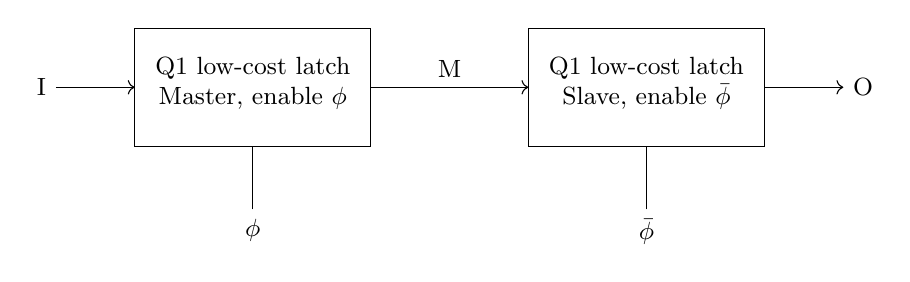
\begin{tikzpicture}[font=\small]
\draw(0,0)rectangle(3,1.5);\draw(5,0)rectangle(8,1.5);\node[align=center]at(1.5,.8){Q1 low-cost latch\\Master, enable $\phi$};\node[align=center]at(6.5,.8){Q1 low-cost latch\\Slave, enable $\bar\phi$};\draw[->](-1,.75)--(0,.75);\node[left]at(-1,.75){I};\draw[->](3,.75)--(5,.75);\node[above]at(4,.75){M};\draw[->](8,.75)--(9,.75)node[right]{O};\draw(1.5,-.8)--(1.5,0);\draw(6.5,-.8)--(6.5,0);\node[below]at(1.5,-.8){$\phi$};\node[below]at(6.5,-.8){$\bar\phi$};
\end{tikzpicture}\\Two complete Figure-1 latch cells; each includes input/forward/feedback inverters and a TG.\end{center}
Each rectangle is the complete 10-MOS Figure-1 cell, with both write-strength inequalities applied separately to its feedback pair. A full two-cell realization has 20 MOS; the first clock inverter's complement can supply the second cell's enable. The complete named-net static realization is saved with the verification files. Practical clock overlap, setup/hold and ratioed-write margins require characterization, not assumed zero from the schematic.

\newpage\section*{Question 3: Valid sharing component and strong-zero restoration}
\textbf{(a)} Label the three unlabelled data controls a,b,c only for analysis, from top to bottom. The original $V_{in}$ drives \emph{both} the precharge pMOS and bottom evaluation nMOS. The stored output $V_F$ has the precharge p drain, the top data n drain, and both inverter gate loads:
\[C_F=2C_d+2C_g=2(1+\alpha)C_d.\]
Each of the three internal junctions has one drain plus one source, so each is $C_d+C_s=2C_d$. During evaluation $V_{in}=1$, the footer is ON. Therefore the lowest internal node is grounded. If all three data nMOS are ON, $V_F$ is connected to ground by a valid logic discharge; it is not a floating sharing case.

The largest valid floating component occurs at a=b=1,c=0, linking $V_F$ to the \emph{top two} internal junctions, with total initially low capacitance $4C_d$. Starting with $V_F=V_{dd}$ and those two junctions at zero,
\[\frac{V_{F,shared}}{V_{dd}}=\frac{2C_d+2C_g}{6C_d+2C_g}=\frac{2+2\alpha}{6+2\alpha}.\]
Correct retained-high recognition requires $V_{F,shared}>V_{dd}/2$:
\[2(2+2\alpha)>6+2\alpha\quad\Longrightarrow\quad\boxed{\alpha>1.}\]
The critical boundary/infimum is 1. At $\alpha=1$ the shared voltage equals the switching threshold and gives no high-state margin, so no strict safe minimum is attained at equality. Pooling all three internal nodes would incorrectly give a stronger bound by treating a ground-connected discharge as isolated sharing. During precharge ($V_{in}=0$), the pMOS is ON and restores $V_F$, so that phase is not the isolated retained-high scenario either. This is the stated lumped-capacitance approximation, excluding unprovided body effect, feedthrough and leakage details.

\textbf{(b)} The existing device is a pMOS controlled by C, ON when C=0. It passes a strong high but a threshold-degraded low. A robust completion retains that device, adds an nMOS between X and Y with gate $\bar C$, and generates $\bar C$ using an explicit CMOS inverter. The path is now a transmission gate: when X=C=0, the nMOS is ON with its source at zero and pulls Y strongly to zero. When C=1 both pass devices are OFF, so the previous Y state is unspecified rather than forced.
\begin{center}\begin{tikzpicture}[font=\small]
\draw(0,1)--(1.2,1)node[pos=0,left]{$X$};\draw(1.2,.82)rectangle(1.7,1.18);\draw(1.45,1.18)--(1.45,1.45);\draw(1.45,1.51)circle(.06);\draw(1.45,1.57)--(1.45,1.9)node[above]{$C$};
\draw(0,1)--(0,-.1)--(1.2,-.1);\draw(1.2,-.28)rectangle(1.7,.08);\draw(1.45,-.28)--(1.45,-.75)node[below]{$\bar C$};\draw(1.7,-.1)--(3,-.1)--(3,1);\draw(1.7,1)--(4,1)node[right]{$Y$};\node[right]at(1.8,-.4){added nMOS};\node[right]at(1.8,1.35){existing pMOS};\node[not gate US,draw](i)at(6,1){};\draw(5,1)--(i.input)node[pos=0,left]{$C$};\draw(i.output)--(7,1)node[right]{$\bar C$};
\end{tikzpicture}\\Completion: explicit CMOS control inverter and an nMOS in parallel with the existing pMOS pass device.\end{center}
This adds three MOS (control inverter 2 and parallel nMOS 1) to the existing pass pMOS, four total. It restores both rails without inventing the threshold of a restore inverter. A conventional inverter-at-Y plus nMOS feedback restorer is another possible design only if the weak pMOS-passed low is below that inverter's switching threshold and the feedback can be overwritten. Those device/threshold conditions are not numerically specified here, so the explicit TG completion avoids relying on them.

\newpage\section*{Question 4: NP full-adder operation}
\textbf{(a)} Let z be the unlabelled first dynamic output and w the unlabelled second dynamic output. The first nMOS pull-down implements $AB+C(A+B)=AB+AC+BC=M$, the carry majority. It has a static output inverter, so $z=\bar M$ and $X=M$. The second pMOS charge network is
\[(\bar A+\bar B+\bar C)(\bar z+\bar A\bar B\bar C).\]
After substituting $z=\bar M$, w is 1 for 000,011,101,110: even parity. Its static output inverter gives
\[\boxed{X=AB+AC+BC\ \text{(carry)},\qquad Y=A\mathbin{\oplus}B\mathbin{\oplus}C\ \text{(sum)}.}\]
The source has 20 MOS: first n-dynamic stage 7, static X inverter 2, p-dynamic stage 9 and static Y inverter 2. The raw \emph{z} wire drives the p-stage; its X output inverter is a separate branch. Connecting X instead of z would change the circuit.

\textbf{(b)} During $\phi=0$, the left precharge raises z and the right reset pulls w low: X=0 and Y=1. During $\phi=1$, the left n-stage can only discharge z, and the right p-stage can only charge w. Inputs A/B/C are held stable for evaluation. The falling z is the required direction for the pMOS-controlled next stage. The evaluated functions and reset values are
\begin{center}\begin{tabular}{c|cc|cc}\toprule
ABC&z&w&X&Y\\\midrule
000&1&1&0&0\\001&1&0&0&1\\010&1&0&0&1\\011&0&1&1&0\\
100&1&0&0&1\\101&0&1&1&0\\110&0&1&1&0\\111&0&0&1&1\\\bottomrule
\end{tabular}\end{center}
\begin{center}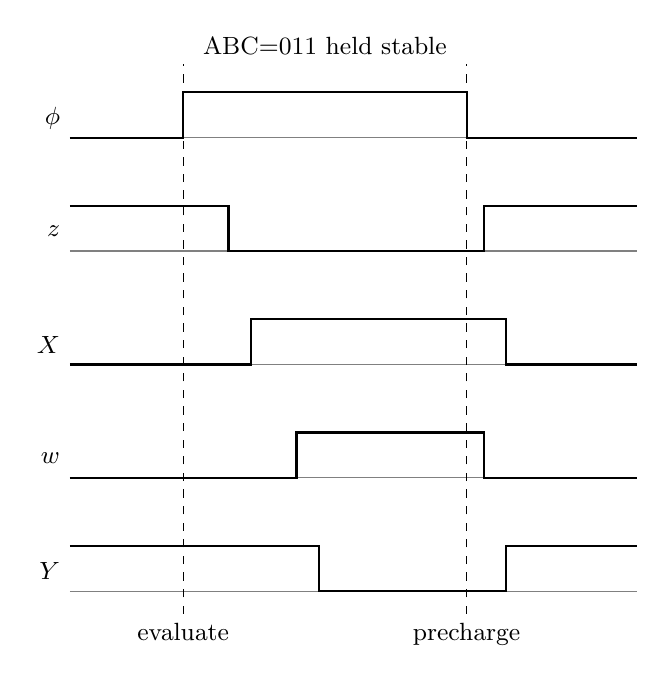
\begin{tikzpicture}[x=.72cm,y=.72cm,font=\small]
\foreach \y/\n in {8/\phi,6/z,4/X,2/w,0/Y}{\node[left]at(0,\y+.35){$\n$};\draw[gray](0,\y)--(10,\y);}
\draw[thick](0,8)--(2,8)--(2,8.8)--(7,8.8)--(7,8)--(10,8);
\draw[thick](0,6.8)--(2.8,6.8)--(2.8,6)--(7.3,6)--(7.3,6.8)--(10,6.8);
\draw[thick](0,4)--(3.2,4)--(3.2,4.8)--(7.7,4.8)--(7.7,4)--(10,4);
\draw[thick](0,2)--(4,2)--(4,2.8)--(7.3,2.8)--(7.3,2)--(10,2);
\draw[thick](0,.8)--(4.4,.8)--(4.4,0)--(7.7,0)--(7.7,.8)--(10,.8);
\draw[dashed](2,-.4)--(2,9.3);\draw[dashed](7,-.4)--(7,9.3);\node[below]at(2,-.4){evaluate};\node[below]at(7,-.4){precharge};\node[above]at(4.5,9.3){ABC=011 held stable};
\end{tikzpicture}\\Illustrative transition order, with no numeric delays assigned. For 000, z/X stay high/low but w rises and Y falls through the direct ABC p-path; for 111, X rises but w/Y remain low/high.\end{center}
The waveforms show transition ordering only, since no resistances, loads or numerical delays are provided. With 000 the p-stage charges through its ABC series branch without waiting for z to fall; with 111 its top parallel p-network is OFF, so w remains low. Repeated A/B/C labels are correlated controls, not separately selectable devices.

\newpage\textbf{Q4(c): a complete n-domino realization.} Standard n-domino outputs rise during evaluation, so a sum XOR cannot be built from only positive A/B/C monotone controls. Supply $\bar A,\bar B,\bar C$ with three explicit CMOS input inverters, and hold both rails stable before/during evaluation. Use independent precharge/footer/output-inverter stages for carry and sum, with the following nMOS PDNs:
\[X:\ AB+AC+BC,\qquad Y:\ \bar A\bar BC+\bar AB\bar C+A\bar B\bar C+ABC.\]
Each product is a series nMOS path and the products are parallel paths, as drawn below. The carry core uses six data nMOS, a precharge pMOS, footer nMOS and CMOS output inverter (10 MOS); sum uses twelve data nMOS plus the same four support devices (16 MOS). Three complementary-input inverters add six, total 32 in this explicit unoptimized design. Output inverter symbols each denote their two CMOS devices with rail sources and common data gate.
\begin{center}\begin{tikzpicture}[scale=.8,font=\scriptsize]
\mos{2.7999999999999994}{5.7}{\phi}{1}\rail{3.0499999999999994}{6.2}{V_{DD}}\draw(3.0499999999999994,5.2)--(3.0499999999999994,4.9);
\draw(0.25,4.9)--(5.85,4.9);
\mos{0.0}{4.1}{A}{0}
\draw(0.25,4.6)--(0.25,4.9);
\mos{0.0}{2.6999999999999997}{B}{0}
\draw(0.25,3.1999999999999997)--(0.25,3.5999999999999996);
\draw(0.25,2.1999999999999997)--(0.25,-.1);
\mos{2.8}{4.1}{A}{0}
\draw(3.05,4.6)--(3.05,4.9);
\mos{2.8}{2.6999999999999997}{C}{0}
\draw(3.05,3.1999999999999997)--(3.05,3.5999999999999996);
\draw(3.05,2.1999999999999997)--(3.05,-.1);
\mos{5.6}{4.1}{B}{0}
\draw(5.85,4.6)--(5.85,4.9);
\mos{5.6}{2.6999999999999997}{C}{0}
\draw(5.85,3.1999999999999997)--(5.85,3.5999999999999996);
\draw(5.85,2.1999999999999997)--(5.85,-.1);
\draw(0.25,-.1)--(5.85,-.1);\draw(3.0499999999999994,-.1)--(3.0499999999999994,-.5);\mos{2.7999999999999994}{-1}{\phi}{0}\gnd{3.0499999999999994}{-1.5}
\node[not gate US,draw](i)at(7.8,4.9){};\draw(5.85,4.9)--(i.input);\draw(i.output)--(8.8,4.9)node[right]{$X$};
\end{tikzpicture}\end{center}\begin{center}\begin{tikzpicture}[scale=.8,font=\scriptsize]
\mos{4.199999999999999}{5.7}{\phi}{1}\rail{4.449999999999999}{6.2}{V_{DD}}\draw(4.449999999999999,5.2)--(4.449999999999999,4.9);
\draw(0.25,4.9)--(8.649999999999999,4.9);
\mos{0.0}{4.1}{\bar A}{0}
\draw(0.25,4.6)--(0.25,4.9);
\mos{0.0}{2.6999999999999997}{\bar B}{0}
\draw(0.25,3.1999999999999997)--(0.25,3.5999999999999996);
\mos{0.0}{1.2999999999999998}{C}{0}
\draw(0.25,1.7999999999999998)--(0.25,2.1999999999999997);
\draw(0.25,0.7999999999999998)--(0.25,-.1);
\mos{2.8}{4.1}{\bar A}{0}
\draw(3.05,4.6)--(3.05,4.9);
\mos{2.8}{2.6999999999999997}{B}{0}
\draw(3.05,3.1999999999999997)--(3.05,3.5999999999999996);
\mos{2.8}{1.2999999999999998}{\bar C}{0}
\draw(3.05,1.7999999999999998)--(3.05,2.1999999999999997);
\draw(3.05,0.7999999999999998)--(3.05,-.1);
\mos{5.6}{4.1}{A}{0}
\draw(5.85,4.6)--(5.85,4.9);
\mos{5.6}{2.6999999999999997}{\bar B}{0}
\draw(5.85,3.1999999999999997)--(5.85,3.5999999999999996);
\mos{5.6}{1.2999999999999998}{\bar C}{0}
\draw(5.85,1.7999999999999998)--(5.85,2.1999999999999997);
\draw(5.85,0.7999999999999998)--(5.85,-.1);
\mos{8.399999999999999}{4.1}{A}{0}
\draw(8.649999999999999,4.6)--(8.649999999999999,4.9);
\mos{8.399999999999999}{2.6999999999999997}{B}{0}
\draw(8.649999999999999,3.1999999999999997)--(8.649999999999999,3.5999999999999996);
\mos{8.399999999999999}{1.2999999999999998}{C}{0}
\draw(8.649999999999999,1.7999999999999998)--(8.649999999999999,2.1999999999999997);
\draw(8.649999999999999,0.7999999999999998)--(8.649999999999999,-.1);
\draw(0.25,-.1)--(8.649999999999999,-.1);\draw(4.449999999999999,-.1)--(4.449999999999999,-.5);\mos{4.199999999999999}{-1}{\phi}{0}\gnd{4.449999999999999}{-1.5}
\node[not gate US,draw](i)at(10.599999999999998,4.9){};\draw(8.649999999999999,4.9)--(i.input);\draw(i.output)--(11.599999999999998,4.9)node[right]{$Y$};
\end{tikzpicture}\end{center}
The evaluated X/Y functions match the original, but conventional n-domino resets both buffered outputs to zero. In particular the reset value of Y differs from the NP source's Y=1; only the evaluation outputs are valid logic results. The input complement inverters must settle before evaluation; an ordinary input transition cannot silently be assumed to produce a legal monotone complementary signal during evaluation.

\newpage\section*{Question 5: 200 MHz pipeline bounds}
The common clock in Figure 5 has no specified skew. At 200 MHz, $T=5\,ns$. Setup gives
\[t_{pcq}+t_{pd}+t_{setup}\le T\quad\Longrightarrow\quad
\boxed{t_{pd}\le5-0.5-1.5=3.0\,ns.}\]
Hold gives
\[t_{ccq}+t_{cd}\ge t_{hold}\quad\Longrightarrow\quad
\boxed{t_{cd}\ge1.0-0.2=0.8\,ns.}\]
Thus the combinational path must satisfy $\boxed{0.8\,ns\le t_{cd}\le t_{pd}\le3.0\,ns}$. These are the minimum contamination-delay requirement and maximum propagation-delay allowance, including any data-path wire delay. Increasing the period does not repair a hold violation. The values are inequalities, not a request to force every path to equal either bound.
\begin{center}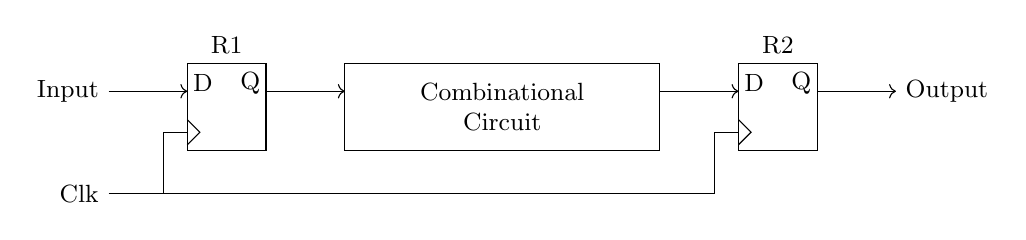
\begin{tikzpicture}[font=\small]
\foreach \x/\name in {0/R1,7/R2}{\draw(\x,-.45)rectangle(\x+1,.65);\node at(\x+.2,.4){D};\node at(\x+.8,.4){Q};\draw(\x,-.38)--(\x+.16,-.22)--(\x,-.06);\node[above]at(\x+.5,.65){\name};\draw(\x-.3,-1)--(\x-.3,-.22)--(\x,-.22);}
\draw(2,.65)rectangle(6,-.45);\node[align=center]at(4,.1){Combinational\\Circuit};\draw[->](-1,.3)--(0,.3);\node[left]at(-1,.3){Input};\draw[->](1,.3)--(2,.3);\draw[->](6,.3)--(7,.3);\draw[->](8,.3)--(9,.3)node[right]{Output};\draw(-1,-1)--(6.7,-1);\node[left]at(-1,-1){Clk};
\end{tikzpicture}\\Figure 5: A pipelined circuit.\end{center}
\section*{Question 6: Eight-MOS literal layout extraction}
The source has four poly crossings in each diffusion row: eight physical MOS. The upper green row lies in n-well and gives pMOS; the lower row gives nMOS. Two well/substrate-tap rectangles at the rails are contacts, not extra transistors. Poly C bends between the rows but remains one C net; Metal-1 crossings without black contacts do not join it. Introduce analysis-only nets v,w,u to name the physical intervals.
\begin{center}\begin{tabular}{c|cc|cc}\toprule
Gate&p left&p right&n left&n right\\\midrule
A&$V_{DD}$&v&$V_{SS}$&F\\B&v&w&F&u\\C&w&F&F&$V_{SS}$\\D&w&v&$V_{SS}$&u\\\bottomrule
\end{tabular}\end{center}
The top long metal connects the right side of A to the right side of D (v); the middle loop connects the right side of B to the left side of D (w). The output F connects the right side of C in the p row, the right side of A and left side of C in the n row. The lower metal loop ties the right side of B to the right side of D (u). Therefore
\[PUN:\ \bar A(\bar B+\bar D)\bar C,\qquad PDN:\ A+C+BD,\]
\[\boxed{F=\overline{A+C+BD}.}\]
\begin{center}\begin{tikzpicture}[x=.92cm,y=.92cm,font=\scriptsize]
\mos{0.0}{0.0}{A}{1}
\node[right]at(0.43,0.0){$\mathrm{PA}$};
\node[above]at(0.25,0.52){$V_{DD}$};
\node[below]at(0.25,-0.52){$v$};
\mos{3.9}{0.0}{B}{1}
\node[right]at(4.33,0.0){$\mathrm{PB}$};
\node[above]at(4.15,0.52){$v$};
\node[below]at(4.15,-0.52){$w$};
\mos{7.8}{0.0}{C}{1}
\node[right]at(8.23,0.0){$\mathrm{PC}$};
\node[above]at(8.05,0.52){$w$};
\node[below]at(8.05,-0.52){$F$};
\mos{11.7}{0.0}{D}{1}
\node[right]at(12.129999999999999,0.0){$\mathrm{PD}$};
\node[above]at(11.95,0.52){$w$};
\node[below]at(11.95,-0.52){$v$};
\mos{0.0}{-2.2}{A}{0}
\node[right]at(0.43,-2.2){$\mathrm{NA}$};
\node[above]at(0.25,-1.6800000000000002){$V_{SS}$};
\node[below]at(0.25,-2.72){$F$};
\mos{3.9}{-2.2}{B}{0}
\node[right]at(4.33,-2.2){$\mathrm{NB}$};
\node[above]at(4.15,-1.6800000000000002){$F$};
\node[below]at(4.15,-2.72){$u$};
\mos{7.8}{-2.2}{C}{0}
\node[right]at(8.23,-2.2){$\mathrm{NC}$};
\node[above]at(8.05,-1.6800000000000002){$F$};
\node[below]at(8.05,-2.72){$V_{SS}$};
\mos{11.7}{-2.2}{D}{0}
\node[right]at(12.129999999999999,-2.2){$\mathrm{ND}$};
\node[above]at(11.95,-1.6800000000000002){$V_{SS}$};
\node[below]at(11.95,-2.72){$u$};
\end{tikzpicture}\end{center}
All eight devices are shown with named channel ends; equal labels are connected. The 16-state conduction check finds exactly one of the PUN or PDN connected to F for every ABCD combination, and confirms the function without changing any source contact.

\newpage\section*{Question 7: Preserve the full complemented function}
In the diagrams below F denotes the requested f, and $\bar F$ denotes its complement. The original overbar covers the \emph{entire} $AB+C+DE$. Let $h=AB+C+DE$; then
\[\boxed{f=\bar h=(\bar A+\bar B)\bar C(\bar D+\bar E).}\]
\textbf{(1) Domino.} Its nMOS PDN must conduct when \emph{f} is true, because the dynamic node Z becomes $\bar f$ and the output CMOS inverter produces f. Use $(\bar A\parallel\bar B)$ in series with $\bar C$ and then $(\bar D\parallel\bar E)$, with the normal precharge/footer. A PDN for h followed by a domino inverter would instead output h and be the wrong polarity. The full core schematic is
\begin{center}\begin{tikzpicture}[x=.92cm,y=.92cm,font=\scriptsize]
\mos{0.0}{0.0}{\bar A}{0}
\node[right]at(0.43,0.0){$\mathrm{NAbar}$};
\node[above]at(0.25,0.52){$Z$};
\node[below]at(0.25,-0.52){$d1$};
\mos{3.9}{0.0}{\bar B}{0}
\node[right]at(4.33,0.0){$\mathrm{NBbar}$};
\node[above]at(4.15,0.52){$Z$};
\node[below]at(4.15,-0.52){$d1$};
\mos{7.8}{0.0}{\bar C}{0}
\node[right]at(8.23,0.0){$\mathrm{NCbar}$};
\node[above]at(8.05,0.52){$d1$};
\node[below]at(8.05,-0.52){$d2$};
\mos{11.7}{0.0}{\bar D}{0}
\node[right]at(12.129999999999999,0.0){$\mathrm{NDbar}$};
\node[above]at(11.95,0.52){$d2$};
\node[below]at(11.95,-0.52){$foot$};
\mos{0.0}{-2.2}{\bar E}{0}
\node[right]at(0.43,-2.2){$\mathrm{NEbar}$};
\node[above]at(0.25,-1.6800000000000002){$d2$};
\node[below]at(0.25,-2.72){$foot$};
\mos{3.9}{-2.2}{\phi}{1}
\node[right]at(4.33,-2.2){$\mathrm{Ppre}$};
\node[above]at(4.15,-1.6800000000000002){$V_{DD}$};
\node[below]at(4.15,-2.72){$Z$};
\mos{7.8}{-2.2}{\phi}{0}
\node[right]at(8.23,-2.2){$\mathrm{Nfoot}$};
\node[above]at(8.05,-1.6800000000000002){$foot$};
\node[below]at(8.05,-2.72){$V_{SS}$};
\mos{11.7}{-2.2}{Z}{1}
\node[right]at(12.129999999999999,-2.2){$\mathrm{Pout}$};
\node[above]at(11.95,-1.6800000000000002){$V_{DD}$};
\node[below]at(11.95,-2.72){$F$};
\mos{0.0}{-4.4}{Z}{0}
\node[right]at(0.43,-4.4){$\mathrm{Nout}$};
\node[above]at(0.25,-3.8800000000000003){$F$};
\node[below]at(0.25,-4.92){$V_{SS}$};
\end{tikzpicture}\end{center}
Named channel ends specify the complete series/parallel graph. Z is the shared precharged node; foot connects only through the clock footer to $V_{SS}$. Add five explicit complementary-input CMOS inverters (p/n gates A, B, C, D or E; common drains at the corresponding complement; rail sources). That is 9 MOS in the domino core and 10 in the complements, 19 total. The complemented controls must be valid and stable at the evaluation boundary or follow the legal domino input monotonicity rule. This answer does not claim inversion is available from positive-only domino inputs for free.

\newpage\textbf{Q7(2): Fully differential.} The f-side pull-down is h (AB series in parallel with C and DE series). The $\bar f$-side pull-down is f, the complement-input network above. Cross-coupled pMOS loads have drains at f/$\bar f$, sources at $V_{DD}$ and gates at the opposite output. One side discharges, and the opposite pMOS restores its complementary high rail. The schematic core is
\begin{center}\begin{tikzpicture}[x=.92cm,y=.92cm,font=\scriptsize]
\mos{0.0}{0.0}{A}{0}
\node[right]at(0.43,0.0){$\mathrm{NA}$};
\node[above]at(0.25,0.52){$F$};
\node[below]at(0.25,-0.52){$ab$};
\mos{3.9}{0.0}{B}{0}
\node[right]at(4.33,0.0){$\mathrm{NB}$};
\node[above]at(4.15,0.52){$ab$};
\node[below]at(4.15,-0.52){$V_{SS}$};
\mos{7.8}{0.0}{C}{0}
\node[right]at(8.23,0.0){$\mathrm{NC}$};
\node[above]at(8.05,0.52){$F$};
\node[below]at(8.05,-0.52){$V_{SS}$};
\mos{11.7}{0.0}{D}{0}
\node[right]at(12.129999999999999,0.0){$\mathrm{ND}$};
\node[above]at(11.95,0.52){$F$};
\node[below]at(11.95,-0.52){$de$};
\mos{0.0}{-2.2}{E}{0}
\node[right]at(0.43,-2.2){$\mathrm{NE}$};
\node[above]at(0.25,-1.6800000000000002){$de$};
\node[below]at(0.25,-2.72){$V_{SS}$};
\mos{3.9}{-2.2}{\bar A}{0}
\node[right]at(4.33,-2.2){$\mathrm{NAbar}$};
\node[above]at(4.15,-1.6800000000000002){$\bar F$};
\node[below]at(4.15,-2.72){$f1$};
\mos{7.8}{-2.2}{\bar B}{0}
\node[right]at(8.23,-2.2){$\mathrm{NBbar}$};
\node[above]at(8.05,-1.6800000000000002){$\bar F$};
\node[below]at(8.05,-2.72){$f1$};
\mos{11.7}{-2.2}{\bar C}{0}
\node[right]at(12.129999999999999,-2.2){$\mathrm{NCbar}$};
\node[above]at(11.95,-1.6800000000000002){$f1$};
\node[below]at(11.95,-2.72){$f2$};
\mos{0.0}{-4.4}{\bar D}{0}
\node[right]at(0.43,-4.4){$\mathrm{NDbar}$};
\node[above]at(0.25,-3.8800000000000003){$f2$};
\node[below]at(0.25,-4.92){$V_{SS}$};
\mos{3.9}{-4.4}{\bar E}{0}
\node[right]at(4.33,-4.4){$\mathrm{NEbar}$};
\node[above]at(4.15,-3.8800000000000003){$f2$};
\node[below]at(4.15,-4.92){$V_{SS}$};
\mos{7.8}{-4.4}{\bar F}{1}
\node[right]at(8.23,-4.4){$\mathrm{PF}$};
\node[above]at(8.05,-3.8800000000000003){$V_{DD}$};
\node[below]at(8.05,-4.92){$F$};
\mos{11.7}{-4.4}{F}{1}
\node[right]at(12.129999999999999,-4.4){$\mathrm{PFbar}$};
\node[above]at(11.95,-3.8800000000000003){$V_{DD}$};
\node[below]at(11.95,-4.92){$\bar F$};
\end{tikzpicture}\end{center}
There are ten data nMOS and two cross-coupled pMOS, 12 core MOS; with five CMOS complement generators, 22 total. The verifier checks all four candidate f/$\bar f$ states for each of the 32 original inputs, confirming one complementary stable state for each.

\textbf{Q7(3): Static CMOS.} Use the five-nMOS h pull-down and its dual five-pMOS pull-up: $(P_A\parallel P_B)$, series $P_C$, series $(P_D\parallel P_E)$. These pMOS gates use the original inputs, since pMOS conduction already complements each control. No input complement generator is needed for this static implementation.
\begin{center}\begin{tikzpicture}[x=.92cm,y=.92cm,font=\scriptsize]
\mos{0.0}{0.0}{A}{0}
\node[right]at(0.43,0.0){$\mathrm{NA}$};
\node[above]at(0.25,0.52){$F$};
\node[below]at(0.25,-0.52){$ab$};
\mos{3.9}{0.0}{B}{0}
\node[right]at(4.33,0.0){$\mathrm{NB}$};
\node[above]at(4.15,0.52){$ab$};
\node[below]at(4.15,-0.52){$V_{SS}$};
\mos{7.8}{0.0}{C}{0}
\node[right]at(8.23,0.0){$\mathrm{NC}$};
\node[above]at(8.05,0.52){$F$};
\node[below]at(8.05,-0.52){$V_{SS}$};
\mos{11.7}{0.0}{D}{0}
\node[right]at(12.129999999999999,0.0){$\mathrm{ND}$};
\node[above]at(11.95,0.52){$F$};
\node[below]at(11.95,-0.52){$de$};
\mos{0.0}{-2.2}{E}{0}
\node[right]at(0.43,-2.2){$\mathrm{NE}$};
\node[above]at(0.25,-1.6800000000000002){$de$};
\node[below]at(0.25,-2.72){$V_{SS}$};
\mos{3.9}{-2.2}{A}{1}
\node[right]at(4.33,-2.2){$\mathrm{PA}$};
\node[above]at(4.15,-1.6800000000000002){$V_{DD}$};
\node[below]at(4.15,-2.72){$p1$};
\mos{7.8}{-2.2}{B}{1}
\node[right]at(8.23,-2.2){$\mathrm{PB}$};
\node[above]at(8.05,-1.6800000000000002){$V_{DD}$};
\node[below]at(8.05,-2.72){$p1$};
\mos{11.7}{-2.2}{C}{1}
\node[right]at(12.129999999999999,-2.2){$\mathrm{PC}$};
\node[above]at(11.95,-1.6800000000000002){$p1$};
\node[below]at(11.95,-2.72){$p2$};
\mos{0.0}{-4.4}{D}{1}
\node[right]at(0.43,-4.4){$\mathrm{PD}$};
\node[above]at(0.25,-3.8800000000000003){$p2$};
\node[below]at(0.25,-4.92){$F$};
\mos{3.9}{-4.4}{E}{1}
\node[right]at(4.33,-4.4){$\mathrm{PE}$};
\node[above]at(4.15,-3.8800000000000003){$p2$};
\node[below]at(4.15,-4.92){$F$};
\end{tikzpicture}\end{center}
The static circuit has 10 MOS and gives f directly. Its complete named-terminal diagram and netlist retain every data device; all 32 original input patterns have exactly one rail path and the required f value.

\section*{Reproducible evidence}
Run \texttt{python verify.py}. The standard-library analytical scripts regenerate the saved CSV/JSON: both latch-write divider inequalities; all dynamic-register phase histories and clock-device polarities; sharing components for all source switch states; completed TG pass truth; full-adder phase truth and complete domino designs; pipeline setup/hold bounds; the literal eight-MOS layout's sixteen truth states; all thirty-two Q7 inputs, sixty-four domino phases and one hundred twenty-eight differential candidate states. These checks are analytical, not SPICE, DRC or extracted timing claims. Editable layout path coordinates, complete netlists, compiler results and page-by-page QA accompany the independent analytical evidence.
\end{document}